\section{Probability interpretation of logistic regression}%Jonathan will input his notes from camera scaned files.
Logistic regression models the probabilities for classification problems with two possible outcomes. It's an extension of the linear regression model for classification problems.
\begin{itemize}
\item Input: d-dimension feature vector $x\in R^{d}$
\item Output: a class or label $l \in\{1, \ldots, k\}$ (how to classify)
\item Example 1: Image classfication:\newline
Given input image $x \in R^{n \times n}$, predict a label for the image. e.g. cat/ dog;
MNIST: $\{0, \ldots, 9\}$; CIFAR-10, $\{0, \ldots, 9\}$
\item Example 2: Binary Classfication:\newline
Given some medical data $x\in R^{d}$(features, like heart pressure, resting heart rate, family history, etc), we try to predict incidence of heart disease. The label will be binary $\{0, 1\}$, called binary classification.
\end{itemize}

\subsection{Logistic Regression Model}
Given input feature vector $x\in R^{n}$, the model predicts a probability distribution over the labels $\{0, \ldots, k\}$. 
$$
\mbox{affine linear map: }Ax+b:\quad R^{n} \rightarrow R^{k} 
$$
with $A\in R^{k \times n}$, $x\in R^{n}$, $b\in R^{k}$.
 $$
 \mbox{softmax} \left( Ax+b\right) : \quad R^{n} \rightarrow R^{k} \xrightarrow{softmax}P\left( \{1, \ldots, k\}\right) 
 $$  
Softmax: 
\begin{enumerate}
\item Input: $y \in \mathbb{R}^{k}=\left(\begin{array}{l}y_{1} \\ \vdots \\ y_{k}\end{array}\right)$
\item Output: Distribution $p(j)=\frac{e^{y_{j}}}{\sum_{i=1}^{n} e^{y_{i}}}$ 
\item Take exponential and normalize
\end{enumerate}

{\bf Logistic Regression Model}: Given input (feature/data) $x \in R^{n}$, we return the distribution softmax  $\left( Ax+b\right) $ where A, b are parameters.
\begin{itemize}
	\item Example 1: Divide data into two classes: parameters are $\vec{a}\in \mathbb{R}^{n}, b \in \mathbb{R}$ 
	$$
	A\in \mathbb{R}^{1\times n},\quad Ax+b\in \mathbb{R}.
	$$
	The probability that the data $x$ belongs to class 1 is 
	$$
	P(1)=\frac{e^{\vec{a}\cdot x+b}}{e^{\vec{a} \cdot x+b}+1},
	$$
	and the probability that the data $x$ belongs to class 2 is
	$$
	P(2)=\frac{1}{e^{\vec{a} \cdot x+ b}+1}.
	$$
	If $\vec{a} \cdot x+ b=0$, $P(1)=	P(2)={1\over 2}$. We don't know how to classify the data lying on the line $\vec{a} \cdot x+ b=0$ as shown in the figure below.
   \begin{figure}[ht!]
  	\centering
  	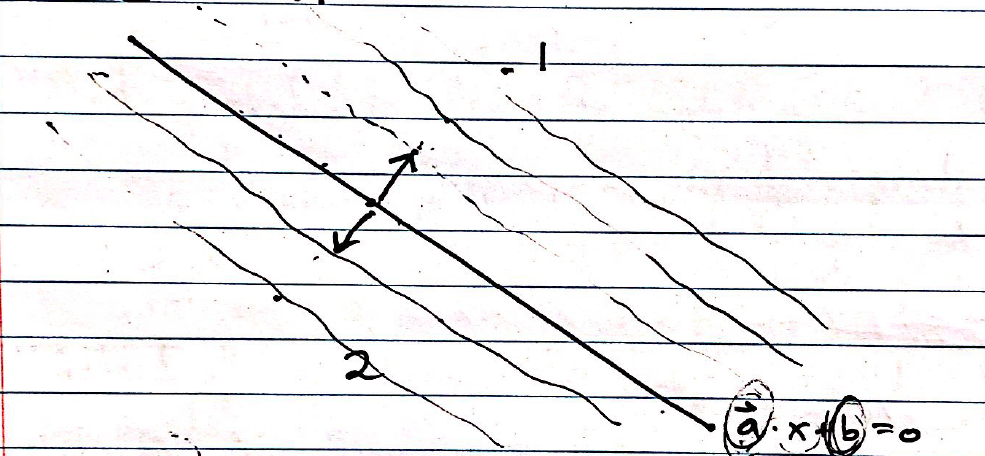
\includegraphics[width=.55\textwidth]{../figures/probabilityLR1.png}  
  \end{figure}
  Note that 
$$
\frac{p(1)}{p(2)}=e^{\vec{a} \cdot x+b},\quad \log \left(\frac{p(1)}{p(2)}\right)=\vec{a} \cdot x+b.
$$
By the above equation, $\vec{a}$ means which feature is important.  \newline
Logarithm of the odds: $ \log \left(\frac{p(1)}{p(2)}\right)$. \newline
Assumption:  $\log \left(\frac{p(1)}{p(2)}\right)$ is linear in the feature vector
\end{itemize}


\subsection{Learning the parameters  $\vec{a}, b$ from data }
Data: feature vectors $x$ and corresponding labels $l$. Given data 
$$
\left\{\left(x_{1}, l_{1}\right), \ldots,\left(x_{n}, l_{1}\right)\right\}=D
$$  
How can we estimate A, b? 

\section{Maximamum Likelihood}
If parameters $A$ and $b$ are known, for any data $x_1\in \mathbb{R}^n$, model gives softmax  $\left( Ax_1+b\right) $ \newline
$$
\frac{1}{\sum_{i=1}^{k} e^{\vec{a_{i}}\cdot x_{i}+b_{i}}} 
\left(\begin{array}{c}e^{\vec{a}_{1}\cdot x_{1} +b_{1}} \\ \vdots \\ e^{a_{k} \cdot x_{1}+b_{k}}\end{array}\right)
=
\left(\begin{array}{c}
p(1)
 \\ \vdots \\ 
p(k)
 \end{array}\right)
$$ 
This means that the probability that the model assigns to $l_{1}$ is
$$
p(l)=\frac{1}{\sum_{i=1}^{k} e^{a_{i}\cdot x_{i}+b_{i}}} \cdot e^{\vec{a}_{l} \cdot x_{1}+b_{l}}
$$  
Instead of considering this probability, we consider its negtive logarithm: \newline
$$
-\log p(l)=\log \left(\sum_{i=1}^{k} e^{a_{i} \cdot x_{i}+b_{i}}\right)-\left(\vec{a}_{l} \cdot x_{1}+b_{l}\right)
$$  
Since data points are independent, so we take product of the probability which leads to the logistic regression loss.\newline
Logistic Regression Loss: 
$$
L_{D}(A, b)=\sum_{(x, l) \in D}\left[\log \left(\sum_{i=1}^{k} a_{i} \cdot x+b_{i}\right)-\left(\vec{a}_{l} \cdot x+b_{l}\right)\right]
$$  
We want to maximize the probability that the model assigns to $l$, that means we need to minimize $-\log p(l)$. So we need to find 
$$
(A, b)=\min _{A, b} L_{D}(A, b).
$$


\section{Basic Statistical Learning Theory}
\begin{itemize}
	\item Goal: Estimate an unknown probability distribution $D$ on a set $X$ from samples $(i,i,d)$ $x_{1}, \ldots, x_{n} \in X$
	\item Introduce a family of distributions $P_{\theta}$ for $\theta \in \Theta$ and try to choose $\theta$ to "match" the samples.
	\begin{itemize}
		\item Maximum Likelihood Estimate: Choose $\theta$ to maximize the probability of the samples.
		\item Example: Let $X=R$, have some samples $x_{1}, \ldots, x_{n}$ drawn from a distribution D, say $P_{\theta}$ is a Gaussian with variance 1, centered at $\theta \in \mathbb{R}=\Theta$, i.e. density  $p_{\theta}(x)=\frac{1}{\sqrt{2 \pi}} e^{-(x-\theta)^{2} / 2}$ 
		
		   \begin{figure}[ht!]
		  	\centering
		  	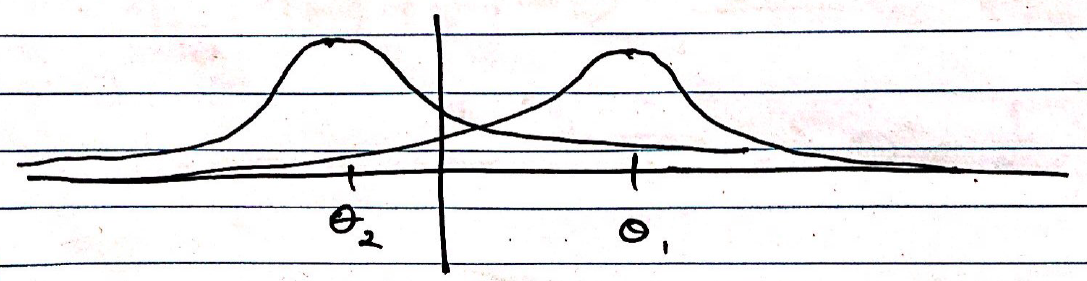
\includegraphics[width=.55\textwidth]{../figures/probabilityLR2.png}  
		  \end{figure}
		\item Use the samples to find the center $\theta$.
	\end{itemize}
\end{itemize}

\subsection{Maximum Likelihood Estimate(MLE)}
\begin{itemize}
	\item Given $\theta \in \Theta (=\mathbb{R}$ for this example), what is the probability of the data $\left\{x_{j}\right\}_{j=1}^{n}$?
	\begin{itemize}
		\item Samles independent: Likelihood function(as a function of $\sigma$) 
		$$
		P_{\theta}\left(\left\{x_{j}\right\}_{j=1}^{n}\right)=\prod_{j=1}^{n} p_{\theta}\left(x_{j}\right)
		=\frac{1}{(\sqrt{2 \pi})^{n}}\prod_{j=1}^{n} e^{-\left(x_{j}-\theta\right)^{2} / 2}
		=\frac{1}{(2 \pi)^{n/ 2}} e^{-\sum_{j=1}^{n}\left(x_{j}-\theta\right)^{2} / 2}
		$$
		\item MLE: Choose $\theta$ to maximize this!
		\item Often it's useful to consider log likelihood function $\log \left(P_{\theta}\left(\left\{x_{j}\right\}_{j=1}^{n}\right)\right) $  
		$$
		\begin{aligned} \theta^{*}= \operatorname{argmax} _{\theta \in \Theta}\log \left(P_{\theta}\left(\left\{x_{j}\right\}_{j=1}^{n}\right)\right) \\
		\left(\operatorname{argmin} _{\theta \in \Theta}-\log \left(P_{\theta}\left(\left\{x_{j}\right\}_{j=1}^{n}\right)\right)\right) \end{aligned}
		$$
	\end{itemize}
     \item For this example: 
     $$
     \log \left(P_{\theta}\left(\left\{x_{j}\right\}_{j=1}^{n}\right)\right)=-\log (2 \pi) \cdot\left(\frac{n}{2}\right)-\sum_{j=1}^{n} \frac{\left(x_{j}-\theta\right)^{2}}{2}
     $$ 
     $$
     \theta^{*}=\operatorname{argmin}_{\theta \in \mathbb{R}} \sum_{j=1}^{n} \frac{\left(x_{j}-\theta\right)^{2}}{2}.
     $$
     $$
      \theta^{*}=\frac{1}{n} \sum_{j=1}^{n} x_{j}.
      $$
     
     	   \begin{figure}[ht!]
       	\centering
       	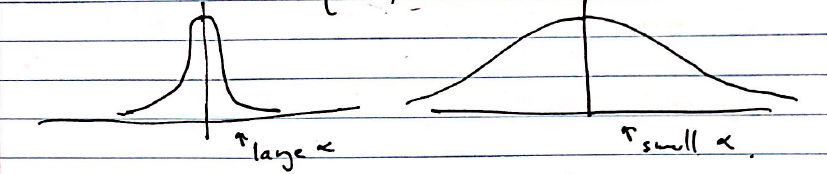
\includegraphics[width=.55\textwidth]{../figures/probabilityLR3.png}  
       \end{figure}
\end{itemize}

\section{Classfication/ Logistic Regression}
\begin{itemize}
	\item For Classification: X is feature space and Y is label space
	$$
	\widetilde{X}=X \times Y
	$$
	\item We have samples $\left\{\left(x_{j}, y_{j}\right)\right\}_{j=1}^{n}$
	\item Suppose that D is an unknown distribution on $\widetilde{X}$, but we're only trying to estimate $D_{Y|X}$ as a function of X. (Given the feature $X$, what is the possible label.)
	\item Introduce parameters $\theta\in \Theta$, we define $p(y|x, \theta)$ (called the model)
	\item Now choose $\theta$ to match the data $\left\{\left(x_{j}, y_{j}\right)\right\}_{j=1}^{n}$
	\item MLE: 
	\begin{align*}
	\theta^{*}&=\operatorname{argmax}_{\theta \in\Theta} p\left(\left\{y_{i}\right\}_{j=1}^{n} |\left\{x_{j}\right\}_{j=1}^{n}, \theta\right)\\
	&=\operatorname{argmax}_{\theta \in\Theta}  \prod_{j=1}^{n} p\left(y_{j} | x_{j}, \theta\right)   \\
	&=\operatorname{argmin}_{\theta \in\Theta}  \sum_{j=1}^{n}-\log \left(p\left(y_{j} | x_{j}, \theta\right)\right)
	\end{align*}
	\item Example: Logistic Regression:
	\begin{itemize}
		\item Model 
		$$
		p(y | x, \theta)=p(y | x, w, b)
		$$
		with $W\in \mathbb{R}^{d\times d}$ and $b\in \mathbb{R}^k$ (parameters for affine linear map)
		\item d: dimension of features, i.e. number of pixels
		\item k: number of classes
	\end{itemize}
$$
p(y | x, w, b)=\mbox{ softmax} \left( W x+b\right)=\frac{1}{\sum_{i=1}^{k} e^{w_{i}\cdot x+b_{i}}}\left(\begin{array}{c}e^{w_{1}\cdot x +b_{1}}  \\ \vdots \\ e^{w_{k} \cdot x +b_{k}}\end{array}\right)
$$
\item Need to calculate:
\begin{equation}\label{eq:pp}
\begin{split}
&-\log \left(p\left(y_{i} | x_{i}, w, b\right)\right)\\
&=-\log \left(\frac{1}{e^{w  x_i+b} \cdot \mathbb{I}} e^{w x_i+b} \cdot y_{i}\right)\\
&=\log \left(e^{w x_i  +b} \cdot 1\right)-\log \left(e^{w x_i+b} \cdot y_{i}\right)
\end{split}
\end{equation}
with $y_i=(0,\cdots, 0,1,0,\cdots, 0)$(only the $i$-th entry is 1, all others are 0) and all the entries of $\mathbb{I}$  are 1.
$$
(w, b)^{*}=\underset{w,b}{\operatorname{argmin}} \sum_{i=1}^{n} \log \left(e^{wx_{i}+b} \cdot \mathbb{I}\right)-\log \left(e^{wx_{i}+b} \cdot y_{i}\right)
$$
\end{itemize}

\section{Bayesian Approach to Machine Learning}
\subsection{Goal}
\begin{itemize}
	\item Goal: Estimate an unknown distribution on X from data $\left\{x_{j}\right\}_{j=1}^{n}$
	\begin{itemize}
		\item Build a model 
	    \begin{itemize}
	    	\item Set of parameters $\Theta$
	    	\item Family of distribution on X, 
		$$p(x|\theta)\quad \mbox{with}\quad \theta \in \Theta $$
	    	\item Prior distribution on the parameters $\Theta$, 
		$$
		q(\theta).
		$$
	    \end{itemize}
    \item Use Bayes' Law 
    $$
    p(\theta|x) p(x)=p(x \  and \   \theta )=p(x | \theta) p(\theta)
    $$
    \item Recall if $A_{1} , A_{2}$ are events:    
    $$
    p\left(A_{1} | A_{2}\right)=\frac{P\left(A_{1} \cap A_{2}\right)}{P\left(A_{2}\right)}
    $$
    $$
    p(\theta | x)=\frac{p(x | \theta) q(\theta)}{p(x)}
    $$
    $$
    p(\theta |x) \sim p(x | \theta) q(\theta)
    $$
    where $p(\theta |x)$ is the posteriori distribution, $q(\theta)$ is the prior distribution and $p(x | \theta)$ is the likelihood function.
	\end{itemize}
\item Stant with: prior $q(\theta)$  
\item Add data $x$, replace $q$ with the posterior
 $$
 p(\theta | x) \sim p(x | \theta) q(\theta)
 $$
\item More data: multiply by likelihood function and then normalize
\item Left with a posterior distribution
     \begin{itemize}
	\item Sample from posterion distribution to approximate
	$$
	P_{pred}(x)=\int_{\Theta} p(x | \theta) p(\theta) d \theta
	$$ 
	\item Choose $\theta $ to maximize posterior distribution  
	\begin{align*}
	\theta^{*}&=\arg \max _{\theta \in \Theta} p(\theta|x)\\
 &=\arg \min _{\theta \in \Theta}-\log p(\theta|x)\\
&=\arg \min _{\theta \in \Theta}-\log (p(x | \theta))-\log (q(\theta))+\log (p(x))\\
&=\arg \min _{\theta \in \Theta}-\log (p(x | \theta))-\log (q(\theta))
\end{align*}
where $-\log (p(x | \theta))$ is the negative log likelihood and $ -\log (q(\theta))$ is the regularization coming from prior.
    \end{itemize}
\subsection{Example: Image  Classification/ Logistic Regression}
\item Images $x \in X=\mathbb{R}^{d}$
\item Labels $y \in Y=\left\{e_{1}, \ldots, e_{k}\right\}$ with $k$ is the dimension of labels
\item Data $\left\{(x_{j},y_{j})\right\}_{j=1}^{n}$
\item Model $\theta=(W, b) \in \mathbb{R}^{k \times d} \times \mathbb{R}^{k}$. By \eqref{eq:pp},
$$
p(y | x, \theta)=\frac{e^{Wx+b} \cdot y}{e^{Wx+b} \cdot \mathbb{I}}
$$
\item Prior distribution: suppose it is a Gaussian,
$$
q(W, b)=C e^{-\alpha\left(\left\|W\right\|_{2}^{2}+ \left\|b\right\|_{2}^{2}\right)}
$$

     	%   \begin{figure}[ht!]
%  	\centering
%  	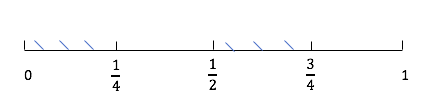
\includegraphics[width=.35\textwidth]{../figures/probability1.png}  
%  \end{figure}

\begin{itemize}
	\item Calculate the posterior: here $q(W,b)=p(W, b|x)$,
	$$
	p(W, b | x, y)=\frac{p(y | x, W, b) p(W, b|x) }{p(y | x)} 
	$$
	$$
	p(y | x)=\int_{\Theta} p(y|x, W, b) q(W, b) d \theta
	$$
	\begin{align*}
	(W, b)^{*}&=\underset{W,b}{\arg \min }-\log \left( p\left(W, b |\left\{x_{j},y_{j}\right\}_{j=1}^{n}\right)\right) \\
&=\underset {W,b}\arg  \min -\log \left( p\left(\left\lbrace y_{j}\right\rbrace _{j=1}^{n} | \left\lbrace x_{j}\right\rbrace _{j=1}^{n}, W, b\right)\right)-\log (q(W, b))\\
&=\underset {W,b}\arg  \min	-\log \left(\prod_{i=1}^{n} p\left(y_{j} | x_{j}, W, b\right)\right)-\log (q(W, b))\\
&=\underset{W, b}{\operatorname{argmin}} \sum_{j=1}^{n} \log \left(e^{Wx+b} \cdot \mathbb{I}\right)-\log \left(e^{Wx_j+b} \cdot y_{j}\right)+\alpha\left(\|W\|_{2}^{2}+\| b\|_{2}^{2}\right).
	\end{align*}


\end{itemize}

\end{itemize}




%\includepdf{HandWrittenNotes/LR1.pdf}
%\includepdf{HandWrittenNotes/LR2.pdf}
%\includepdf{HandWrittenNotes/LR3.pdf}
%\includepdf{HandWrittenNotes/BasicSLT1.pdf}
%\includepdf{HandWrittenNotes/BasicSLT2.pdf}
%\includepdf{HandWrittenNotes/BasicSLT3.pdf}
%\includepdf{HandWrittenNotes/BasicSLT4.pdf}
%\includepdf{HandWrittenNotes/Bayesian2.pdf}
%\includepdf{HandWrittenNotes/Bayesian1.pdf}
%\includepdf{HandWrittenNotes/Bayesian3.pdf}
%\includepdf{HandWrittenNotes/Bayesian4.pdf}